\chapter{Variational methods in Image Processing}
\label{chapter:variational-methods-in-image-processing}

\section{Inverse problems}
%In the music world, nothing is as complex as an orchestra score. You have plenty of instruments following different tones, dynamics, intensities, rhythms and so on. But no matter the complexity, given the orchestra score a software can reproduce with perfection the piece of music. It is a totally  different story if you ask it to create the orchestra score from an audio file. Reading the score is a forward problem, and creating the score is an inverse problem.

An archaeological museum decided to digitize all its collection and make them available for digital visits over the internet. The chosen method of digitization consists into take a set of pictures, in different camera positions, for each object and then to use a stereo algorithm to assemble all the pieces and create a 3D model of the object. The stereo problem is an \emph{inverse problem}.

Inverse problems are characterized by a degree of \emph{uncertainty} or \emph{lack of information}. The 2D pictures in the problem above miss depth information, that should be \emph{inferred} by the stereo algorithm. On the other hand, if the shape geometry was known, e.g., the values of mean curvature were known for every infinitesimal point of the shape, then constructing a digital 3D representation would be a \emph{forward problem}. 

Inverse problems are ubiquitous in science. We can find inverse problems in several branches of mathematics~\cite{kirsch96}, geophysics~\cite{zhdanov15}, natural language processing~\cite{stroppa05}, astronomy~\cite{lucy94} and the list goes on. The image processing field itself field is plenty of examples of inverse problems~\cite{bertero98}, some of them listed in table~\cref{ch1:tab:inverse-problems-list}. In fact, a great part of real world applications consists into infer parameters of some model, i.e., an inverse problem. In~\cref{ch1:tab:inverse-problems-list} we list some examples of inverse problems and its corresponding direct problem version.

\begin{table}
\renewcommand{\arraystretch}{1.5}
\footnotesize
\begin{tabular}{|m{7cm}|m{7cm}|}
\hline
\multicolumn{1}{|c|}{\textbf{Inverse problem}} & \multicolumn{1}{c|}{\textbf{Forward problem}} \\
\hline
\textbf{Projection}: Compute vector $v \in \mathbb{R}^3$ which projection is $P(v) \in \mathbb{R}^2$ & Compute the projection $P(v) \in \mathbb{R}^2$ of vector $v \in R^3$\\
\hline
\textbf{Parameters inference}: Given a set of observations $\Gamma$, infer the parameters $(\mu,\sigma)$ of the Gaussian distribution that describes $\Gamma$ & Given a random variable $X$ following a Gaussian distribution with parameters $(\mu=0,\sigma=1)$, compute the probability $P(X \leq 0.42)$\\
\hline
\textbf{Image denoising}: Given noisy image $\widetilde{\vec{I}}$, compute the original image $\vec{I}$, i.e., the image without noise & Add some random noise to a given image $\vec{I}$ to produce noisy image $\widetilde{\vec{I}}$\\
\hline
\textbf{Image inpainting}: Given image $\widetilde{\vec{I}}$ with a missing patch, reconstruct the removed patch & Remove a patch from image $\vec{I}$ \\
\hline
\textbf{Image segmentation}: Given image $I$, find the labeled partition $\mathcal{I}$ & Given a labeled partition $\mathcal{I}$ of some image $I$, assemble the pieces to create image $I$\\
\hline
\end{tabular}
\caption{Examples of inverse problems and its direct versions. Inverse problems are characterized by uncertainty and parameter inference. }
\label{ch1:tab:inverse-problems-list}
\end{table}

In mathematics, uncertainty is very often translated in to ill-posed problems. An ill-posed problem is a problem that is not well-posed. A well-posed problem, on the other hand, must respect the two conditions below.

\begin{enumerate}
\item{A solution exists and it is unique;}
\item{The solution changes continuously with its parameters}
\end{enumerate}



Generally speaking, an inverse problem is ill-posed. In order to solve ill-posed problems one should include additional information, i.e., create assumptions over the properties of searched solution. For example, one may assume that vector $v$ is at some distant $d$ of $P(v)$ for the projection problem. The solution set, in this case, is restricted to two. The process of including additional information in ill-posed problems is called \emph{regularization} and its goal is to transform ill-posed problems in well-posed ones. 

\section{Image model}
As remarked in the previous section, inverse problems involve some level of uncertainty about the solution. In order to solve an ill-posed problem we need to regularize it by including additional information, or assumptions. To simplify notation, we limit our discussion to grayscale images, the concepts being extendable to multichannel images. It is convenient to have in mind two different representations of an image. \\

\begin{center}
\begin{tabular}{rl}
	Continuous: & $f_I: \Omega \subset \mathbb{R}^2 \rightarrow \mathbb{U}$ \\
	Discrete: & $I \in \mathbb{F}^{m \times n}$,
\end{tabular}
\end{center}

where $\mathbb{F}$ is a finite set. In this thesis, we define such set as

\begin{align}
	\mathbb{F} &= \{ \frac{i}{255} \; | \; i \in \mathbb{N}, i \leq 255 \}.
\end{align}

The discrete representation is interpreted as a sampling of $m \times n$ elements (pixels) of the continuous function $f_I$. 

\section{Image denoising}
Image denoising is one of the classical problems in image processing. Given an image $\vec{\widetilde{I}}$ corrupted by some noise, the problem consists in to recover the original image $\vec{I}$. Besides the quality improvement of the devices over the years, the denoising task is still an important task in satellite and medical image processing.

\subsection{Bayesian rationale}
The maximum a posteriori method was first introduced in the image processing community in the work of~\cite{geman84}. We reproduce it here the rational for image denoising.

Image denoising is an inverse problem and we need to make some assumptions in order to advance in its solution. We assume

\begin{enumerate}
	\item{The noisy image $\vec{\widetilde{I}}$ is obtained by adding a normal Gaussian noise ($\mu=0,\sigma=1$) to the original image, i.e., 
		\begin{assumption}
		\begin{align}
			\vec{\widetilde{I}} &= \vec{I} + \vec{N},
		\label{ch1:denoising-assumption-1}
		\end{align} 
		\end{assumption}
where $\vec{N}$ is a $(m \times n)$ matrix of random variables $\vec{N}_{i,j}$ and $Pr\big( \vec{N}_{i,j} = n \big) = \frac{1}{\sqrt{2\pi}}exp( \frac{n^2}{2} )$.		
	}
	\item{Given some function $\rho$, a candidate image $\vec{C}$ has probability
	
	\begin{assumption}
	\begin{align}
		Pr(\vec{C}) = exp(-\rho(\vec{C})).
		\label{ch1:denoising-assumption-2}
	\end{align}	 
	\end{assumption}
	}
\end{enumerate}

%If we want to be precise, the sum operator in~\cref{ch1:denoising-assumption-1} should be redefined to be a closed operator in $\mathbb{F}^{m \times n}$. We skip this definition by arguing that because of the symmetry of the Gaussian distribution the computation of the probabilities that follows remains the same.

 We estimate the unknown original image $\vec{I}$ as the image $\vec{\widehat{I}}$ that is more likely to occur. Applying Bayes' theorem we obtain

\begin{align}
	\vec{\widehat{I}} & = \argmax _{\vec{C}}{Pr(\vec{C} \; | \;\vec{\widetilde{I}})} = \argmax _{\vec{C}} \frac{Pr(\vec{\widetilde{I}} \; | \; \vec{C})Pr(\vec{C})}{Pr(\vec{\widetilde{I}})}.
	\label{ch1:eq:probability-maximization}
\end{align}

We have already all the elements to expand~\cref{ch1:eq:probability-maximization}. The probability of having the corrupted image $\vec{\widetilde{I}}$ given a candidate image $\vec{C}$ is derived from~\cref{ch1:denoising-assumption-1}, i.e.,

\begin{align}
	Pr(\vec{\widetilde{I}} \; | \; \vec{C}) &= Pr( \vec{N} = \vec{\widetilde{I}} - \vec{C} ) = \frac{1}{\sqrt{2\pi}}exp\Big(- \frac{ \norm{\vec{\widetilde{I}} - \vec{C} }^2}{2} \Big).
	\label{ch1:eq:probability-corrupted-image-given-original}
\end{align}

The denominator term is computed as the joint probability

\begin{align}
	Pr(\widetilde{\vec{I}}) &= \sum_{\vec{J} \in \mathbb{F}^{m \times n}}{Pr(\vec{\widetilde{I}}\;|\; \vec{J})Pr(\vec{J})} = \frac{1}{\sqrt{2 \pi}}\sum_{\vec{J} \in \mathbb{F}^{m \times n}}{exp\bigg(-\frac{1}{2}\norm{\widetilde{\vec{I}}-\vec{J}}^2 - \rho(\vec{J})}\bigg).
	\label{ch1:eq:joint-probability}
\end{align}

Substituting~\cref{ch1:eq:probability-corrupted-image-given-original,ch1:eq:joint-probability} in~\cref{ch1:eq:probability-maximization} we obtain

\begin{align}
	\vec{\widehat{I}} & = \argmax _{\vec{C}} \frac{1}{\sqrt{2\pi}} \frac{exp\Big(- \frac{1}{2}\norm{\vec{\widetilde{I}} - \vec{C}}^2 - \rho(\vec{C}) \Big) }{ \sum_{\vec{J} \in \mathbb{F}^{m \times n}}{exp\bigg(-\frac{1}{2}\norm{\widetilde{\vec{I}}-\vec{J}}^2 - \rho(\vec{J})}\bigg) }
	\label{ch1:eq:probability-maximization-expanded}
\end{align}

Finnaly, solving~\cref{ch1:eq:probability-maximization-expanded} is equivalent to solve

\begin{align}
	\vec{\widehat{I}} &= \argmin _{\vec{C}} \frac{1}{2}\norm{\vec{\widetilde{I}} + \vec{C}}^2 + \rho(\vec{C}).
	\label{ch1:eq:minimization-form}
\end{align}

The first term appears so often in image processing that it has a special name: \emph{data fidelity}. In the denoising problem, the data fidelity term appeared as a consequence of the Gaussian noise model assumption. The second term is also a regularization term and it favors images that respect some desirable property for the problem to be solved. A popular one for denoising is to assume that the image is piecewise smooth, i.e., the image is composed of closed regions with smooth variations in its interior and strong discontinuities in their boundaries. 
%We can follow this reasoning for each new assumption we made. The consequence being an additional term in~\cref{ch1:eq:minimization-form}.

\subsection{Tikhonov regularization}
\label{ch1:subsec:tikhonov-regularization}
The classical way to optimize~\cref{ch1:eq:minimization-form} is to shift it to a continuous setting, analytically derive optimization properties and then use this properties to solve the problem in a discrete setting. The continuous reformulation of~\cref{ch1:eq:minimization-form} consists in to optimize the energy functional below

\begin{align}
	f_{\vec{\widehat{I}}} &= \argmin_{f} F(f) = \frac{1}{2} \int_{\Omega}{ \norm{ f_{\vec{\widetilde{I}}} - f}^2dx} + R(f),
	\label{ch1:eq:variational-formulation}
\end{align}

where $R$ is a functional derived from the choice of $\rho$. A popular choice for $R$ is to define it as the $L2$ norm of $\nabla f$, also called the \emph{Tikhonov} regularization term.~\cref{ch1:eq:variational-formulation} is rewritten as

\begin{align}
	f_{\vec{\widehat{I}}} &= \argmin_{f} F(f) = \frac{1}{2} \int_{\Omega}{ \norm{ f_{\vec{\widetilde{I}}} - f}^2dx} + \int_{\Omega}{ \norm{ \nabla f }^2 dx }.
	\label{ch1:tikhonov-formulation}
\end{align}

\subsubsection{Euler-Lagrange equation}

We can establish some necessary optimization conditions for~\cref{ch1:tikhonov-formulation} by deriving its Euler-Lagrange equation. Assume that function $g$ minimizes functional $F$, i.e.,

\begin{align*}
	g &= \argmin_{f}{F(f)}.
\end{align*}

Further, assume that there exists a function $w$ such that $w(x)=0,\, \forall x \in \partial \Omega$. Define the function $h$ as

\begin{align*}
	h(\epsilon) &= F(g+\epsilon w)
\end{align*}

Therefore, $h$ achieves an extreme value in $\epsilon=0$. Thus,

\begin{align*}
	0 = \frac{dh}{\partial \epsilon}_{| \epsilon=0} &= \frac{d}{\partial \epsilon}_{| \epsilon=0} \frac{1}{2} \int_{\Omega}{ \norm{f_{\vec{\widetilde{I}}} - g - \epsilon w}^2 + \norm{ \nabla (g + \epsilon w) }^2} \\
	&= _{| \epsilon = 0} \frac{1}{2} \int_{\Omega}{ 2\norm{ f_{\vec{\widetilde{I}}} - g - \epsilon w}\frac{(f_{\vec{\widetilde{I}}} - g - \epsilon w) }{\norm{f_{\vec{\widetilde{I}}} - g - \epsilon w}}w + 2\norm{ \nabla (g + \epsilon w) }\frac{(\nabla g + \epsilon w)}{\norm{ \nabla (g + \epsilon w) }}\nabla w} \\
	&= \int_{\Omega}{ (f_{\vec{\widetilde{I}}} - g)w + (\nabla g)\nabla w}. 	
\end{align*}

Applying integration by parts and using the fact that $w(x)=0,\; \forall x \in \partial \Omega$.

\begin{align*}
		0 &= \int_{\Omega} ( f_{\vec{\widetilde{I}}} - g - \Delta g )w
\end{align*}

Since $w$ could be any function, we can write

\begin{align}
	f_{\vec{\widetilde{I}}} - g - \Delta g &= 0
	\label{ch1:eq:variational-necessary-condition}
\end{align}


Therefore, if $g$ is a minimum of~\cref{ch1:eq:variational-formulation}, then it respects ~\cref{ch1:eq:variational-necessary-condition}. ~\cref{ch1:eq:variational-formulation} can be proven to be convex. Hence, given an initial solution $f$, one can execute a descent method (gradient descent, for example) to find the minimum of~\cref{ch1:eq:variational-formulation}. In practice, ~\cref{ch1:eq:variational-formulation} is discretized using the samplings $\vec{\widehat{I}}, \vec{\widetilde{I}}$ of $f_{\vec{\widehat{I}}},f_{\vec{\widetilde{I}}}$ and a finite differences scheme is defined to estimate the Laplacian $\Delta$.

The Tikhonov term favors images with smooth variations in color, but the smoothness is not restricted to the interior of regions. Thus, Tikhonov tends to obfuscate the discontinuities set and the image appears to be blurred (see~\cref{ch1:fig:denoising-results}). Nonetheless, Tikhonov term is attractive due to its optimization properties.

\begin{figure}
\subfloat[Original]{
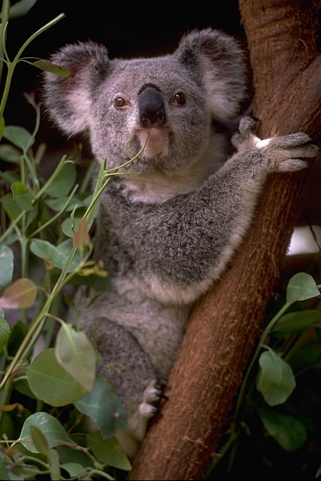
\includegraphics[scale=0.38]{figures/chapter2/denoising/coala-original.png}
}%
\subfloat[Noisy]{
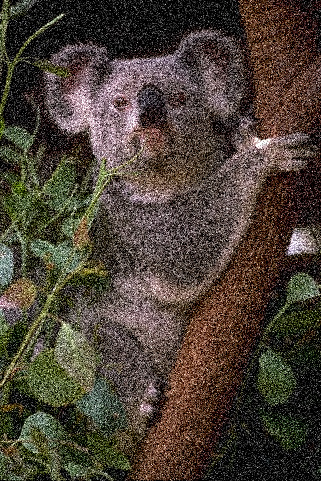
\includegraphics[scale=0.38]{figures/chapter2/denoising/coala-noise.png}
}%
\subfloat[Tikhonov]{
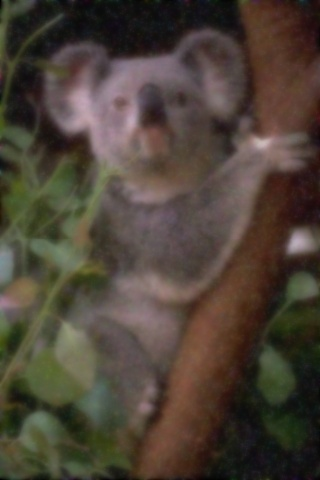
\includegraphics[scale=0.38]{figures/chapter2/denoising/coala-tikhonov.png}
}%
\subfloat[Total Variation]{
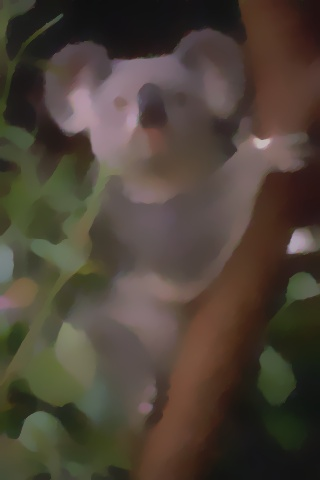
\includegraphics[scale=0.38]{figures/chapter2/denoising/coala-chambolle.png}
}%
\caption{Denoising algorithms results for the Tikhonov and Total variation regulararization terms.}
\label{ch1:fig:denoising-results}
\end{figure}


\subsection{Total variation regularization}
An alternative to Tikhonov regularization is to use the so called total variation of the image function. The problem to be minimized is then defined as

\begin{align}
	f_{\vec{\widehat{I}}} &= \argmin_{f} \frac{1}{2} \int_{\Omega}{ \norm{ f_{\widetilde{I}} - f}^2dx} + \int_{\Omega}{ \norm{\nabla f} dx}.
\end{align}

The $L1$ norm favors smooth interiors and it is less aggressive in the boundaries than the Tikhonov regularization. Moreover, there are efficient algorithms to solve it~\cite{rudin92,chambolle04,beck09}.


\section{Image segmentation}
Given an image $\vec{I}$, we wish to compute the partition $\mathcal{I}$ of $\vec{I}$ such that each member $\mathcal{I}_j$ of $\mathcal{I}$ correspond to the set of pixels identified with some object of $\vec{I}$. In this section we present three paradigms that frequently appear in the literature while coping with variational problems in image processing: Parametric curve evolution (active contours); level-set method (Chan-Vese); and convexification (). All the presented models can be seen as a specification of the classical Mumford-Shah model.

\subsection{Mumford-Shah}
The $L2$-norm regularization has nice optimization properties, but it does not preserve the discontinuities presented in the image edges. This effect is attenuate using a $L1$-norm, but it it not sufficient to avoid blurred edges. The \emph{Mumford-Shah} functional~\cite{mumford89} handles this issue by incorporating the edges in its formulation in the form of a set of discontinuities $\mathcal{K}$ and limiting the $L2$-norm regularization to points in $\Omega \setminus \mathcal{K}$. Moreover, the set $\mathcal{K}$ itself is compelled to be of small length. The Mumford-Shah model consists in to minimize the following functional 


\begin{align}
	(f_{\vec{\widehat{I}}},\mathcal{\widehat{K}}) &= \argmin_{f,\mathcal{K}} \alpha \int_{\Omega}{ \norm{f_{\vec{\widetilde{I}}}-f}dx} + \beta \int_{\Omega \setminus \mathcal{K}}{\norm{\nabla f}dx} + \lambda Per(\mathcal{K})
	\label{ch1:mumford-shah-functional}
\end{align}

The functional can be seen as a model for both denoising and segmentation problems. The function $f_{\vec{\widehat{I}}}$ is the denoising solution and $\mathcal{\widehat{K}}$ is the segmentation solution.~\cref{ch1:mumford-shah-functional} is proven to have a minimizer~\cite{degiorgi89}, and in the case $\mathcal{K}$ is fixed, the minimizer is unique (see chapter 25 of~\cite{bar11}). However, to find a minimizer of~\cref{ch1:mumford-shah-functional} is a challenging task due its non-convexity, in particular the optimization of the discontinuity set $\mathcal{K}$. 

Nonetheless, there exists several approximations to the Mumford-Shah functional. We refer to the phase-field model of~\cite{ambrosio90}; the finite-differences scheme of~\cite{chambolle99}; the level-set method of~\cite{vese02}; and the convex relaxations of~\cite{pock09,strekalovskiy14}. 


\subsection{Active contours}
Active contours or snakes is a supervised method for doing image segmentation. In the original work~\cite{kass88}, an initial parametric curve $c(t) \rightarrow (x(t),y(t))$ is evolved towards the local minimum of the snakes energy

\begin{align}
	F() &= \alpha Length(c) + \beta Smoothness(c) + \gamma Edge(c) \\
	F() &= \alpha \int_{0}^{1}{ \bignorm{ \frac{dc}{\partial t} }^2 dt } + \beta \int_{0}^{1}{ \bignorm{ \frac{d^2c}{\partial t^2} }^2dt} + -\gamma \int_{0}^{1}{ \norm{ \nabla f_I(c(t))}^2 dt}\\
	\label{ch1:eq:snakes-energy}
\end{align}

%\begin{align*}
%	E_{img} &= - \int_c{ \norm{ \nabla f_I(c)}^2 dc}\\
%	&= -\int_{0}^{1}{ \bignorm{ \left(\frac{d f_I}{\partial x}\frac{d x}{\partial t}, \frac{d f_I}{\partial y}\frac{d y}{\partial t} \right)}^2dt }.
%\end{align*}

The length and smoothness regularization term favors curves of smooth variations and  small length. The edge term is the most important for image segmentation, and it forces the curve to stop at regions of high variation of color intensity. A weakness of the model is its inability to change its topology. One needs to initialize several snakes in order to correctly segment a picture with several holes, for example.

The snakes method was devised having an interactive framework in mind. First of all, the user must set the initial curve close to the object to be segmented, and besides that, a set of additional tools as anchor points, repulsion and spring forces are available for online modification of the problem. The user can make use of these tools to conveniently perturb the current solution and force the curve to evolve to the expected local optimum.

The active contours is an influential paradigm for image segmentation and it was particularly popular for segmenting medical images~\cite{mcinerney99}. Variations of the original model include extension to 3D-segmentation~\cite{mcinemey99} and topologically adaptable snakes~\cite{mcinerney95}.

%This approach is also non-
%intrinsic, since the energy depends on the parametriza-
%tion of the curve and is not directly related to the objects
%geometry. As we show in this paper, a kind of “re-
%interpretation” of this model solves these problems.
%See for example (Malladi et al., 1995) for comments
%on other advantages and disadvantages of energy ap-
%proaches of deforming contours, as well as an extended
%literature on snakes.

%Energy minimization x Curve evolution approaches

%In this paper a particular case of the classical en-
%ergy snakes model is proved to be equivalent to find-
%ing a geodesic curve in a Riemannian space with a
%metric derived from the image content. This means
%that in a certain framework, boundary detection can
%be considered equivalent to finding a curve of mini-
%mal weighted length. This interpretation gives a new
%approach for boundary detection via active contours,
%based on geodesic or local minimal distance computa-
%tions.
 
%O modelo do Caselles jah era um modelo do tipo level set
%que ja era capaz de surmontar os obstaculos de uma evolucao
%sem alteracao de topologia, como eh o caso das snakes. 
 
%Solving the problem of
%snakes amounts to finding, for a given set of constants
%α, β, and λ, the curve C that minimizes E. Note that
%when considering more than one object in the image,
%for instance for an initial prediction of C surrounding
%all of them, it is not possible to detect all the objects.
%Special topology-handling procedures must be added.
%Actually, the solution without those special procedures
%will be in most cases a curve which approaches a con-
%vex hull type figure of the objects in the image. In
%other words, the classical (energy) approach of snakes
%can not directly deal with changes in topology.


%This will allow to achieve
%smooth curves in the proposed approach without hav-
%ing the high order smoothness given by β 6= 0 in
%energy-based approaches. 3 Moreover, the second order
%smoothness component in (1), assuming an arc-length
%parametrization, appears in order to minimize the to-
%tal squared curvature (curve known as “elastica”). It is
%easy to prove that the curvature flow used in the new ap-
%proach and presented below decreases the total curva-
%ture (Angenent, 1991). The use of the curvature driven
%curve motions as smoothing term was proved to be very
%efficient in previous literature (Alvarez et al., 1993;
%Caselles et al., 1993; Kimia, —; Niessen et al., 1993;
%Malladi et al., 1994, 1995, —; Sapiro and Tannenbaum,
%1993), and is also supported by our experiments in Sec-
%tion 4. Therefore, curve smoothing will be obtained
%also with β = 0, having only the first regularization
%term. Assuming this (1) reduces to


%Leaving \beta \neq 0 in the active contours lead to a fourth-order
% term in the Euler-Lagrange equation

%The functional in (2) is not intrinsic since it depends
%on the parametrization q that until now is arbitrary.
%This is an undesirable property, since parametrizations
%are not related to the geometry of the curve (or object
%boundary),

%The Euclidean heat flow, what I call the curvature flow,
%
%is well known for
%its very satisfactory geometric smoothing properties
%(Angenent, 1991; Gage and Hamilton, 1986; Grayson,
%1987). (It was extended in (Sapiro and Tannenbaum,
%1993a, b, 1994) for the affine group and in (Olver
%et al., 1994, —; Sapiro and Tannenbaum, 1993) for
%others.) The flow decreases the total curvature as well
%as the number of zero-crossings and the value of max-
%ima/minima curvature.

%It is a shortening and smoothing terms simultaneously.


%This is achieved with the help of the
%mentioned level-set numerical algorithm for curve evo-
%lution, developed in (Osher and Sethian, 1988; Sethian,
%1989) and already used by others for different im-
%age analysis problems (Chopp, 1991; Kimia et al., —;
%Kimmel et al., 1995, —; Kimmel and Sapiro, 1995;
%Sapiro et al., 1993; Sapiro and Tannenbaum, 1993a,
%1995). In this case, the topology changes are automat-
%ically handled without the necessity to add specific
%monitoring on the deforming curve or any heuristic
%criterion.

%This energy is however not intrinsic to the curve geometry, since it
%also depends on the parameterization of the curve. This is why these
%two terms were replaced by length element and curvature to obtain an
%intrinsic energy and define a geometric model [57]. Since it is complex
%to deal with the curvature term, it was removed in that model, as
%well as in the level set approach of Malladi et al. [179]


%The unsigned distance function φ̃ s is the unique
%viscosity solution of the Eikonal equation
%||∇ φ̃ t (x)|| = 1
%and ∀ s ∈ [0, 1], φ̃ t (γ(s)) = 0.
%(3.9)
%This equation can be solved in O(N log(N )) operations on a regular
%grid of N pixels using the Fast Marching algorithm detailed in Section
%2.3

%In the case of noisy images, the initial image is convolved with a Gaussian kernel

%Fethallah Benmansour and Laurent D. Cohen. Fast object segmentation by
%growing minimal paths from a single point on 2D or 3D images. J. Math.
%Imaging Vis., 33(2):209–221, February 2009.

%Vessel segmentation using shortest paths. Top left: original retinal image from
%DRIVE database [199].


%Relation with watershed. If the geodesic distance map U S is ap-
%proximated with morphological operators, as detailed in Section 2.8.1,
%the Voronoi segmentation corresponds to the result of the water-
%shed algorithm initially proposed in [28] and extended for instance
%in [283, 198, 188]. For the watershed algorithm, the set of initial points
%S is usually chosen as the local minima of the map W (x), possibly after
%some smoothing pre-processing.

\subsection{Geometric active contours}
Parametric models as snakes are often criticized because of their non-intrinsic definition, i.e., the energy is not defined in terms of the geometric properties of the contours. That fact difficulties the theoretical analysis of the snakes model, as the evolution of the contour itself depends of the chosen parametrization. In~\cite{caselles93} the authors propose a model based on the mean curvature motion of the level-sets of a $C^2$ function $u$.


Let $u:\Omega \subset \mathbb{R}^2 \rightarrow \mathbb{U}$ be a $C^2$ function. The curvature at its $k$-th level set is given by

\begin{align*}
	\kappa (x,y) &= \nabla \cdot \left( \frac{\nabla u}{\norm{\nabla u}} \right), \quad \forall (x,y) \in \left\{ \; (x,y) \; | \; u(x,y)=k \; \right\}
\end{align*}


We proceed by artificially including a time parameter $t$ at $u$ and compute the steady solution of the flow

\begin{align}
	u(0,x,y) &= u(x,y) \nonumber \\
	\frac{du}{dt} &= g( \norm{\nabla f_I} )\norm{\nabla u}\nabla \cdot \left( \frac{\nabla u}{\norm{\nabla u}}  + v \right),
	\label{ch1:geometric-active-contour}
\end{align}

where $g$ is a non-increasing function that plays the role of an edge-detector, e.g., $g(x) = 1/(1+x)^2$. The function $u$ can be initially defined as a smoothed version of $1 - \chi_C$, where $\chi_C$ is the characteristic function of some set $C \in \Omega $ that contains the objects to be segmented. 

Following~\cref{ch1:geometric-active-contour}, the gray level at some point $(x,y)$ changes proportionally to the curvature of its belonging level set. The constant $v$ forces the change in $u$ to be always positive, i.e., pixels gets lighter, never darker. The term $\norm{\nabla u}$ allows $u$ to evolve only at some neighborhood of the $0$-level-set boundary and the term $g(\norm{\nabla f_I})$ makes the evolution to stop if an edge is reached. At the steady solution of~\cref{ch1:geometric-active-contour} the segmented objects of $\vec{I}$ corresponds to the $0$-level set of $u$.

Differently from the snakes, the geometric active contours handle changes in topology of the initial curve. In figure~\cref{ch1:fig:comparison-curve-evolution}, the initial $0$-level set of $u$ splits in three disjoint sets at the steady solution of~\cref{ch1:geometric-active-contour}. However, the geometric active contour models cannot segment objects with holes without including a region-based term~\cite{chen06}.

\begin{figure}
\center
\subfloat[Active contours]{
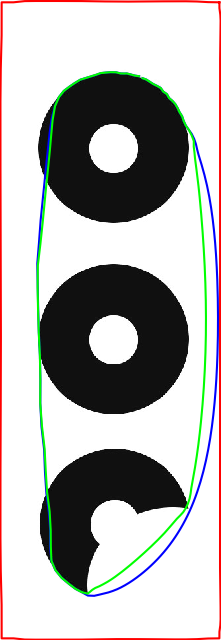
\includegraphics[scale=0.5]{figures/chapter2/segmentation/active-contour.png}
}\hspace{2em}%
\subfloat[Geometric active contours]{
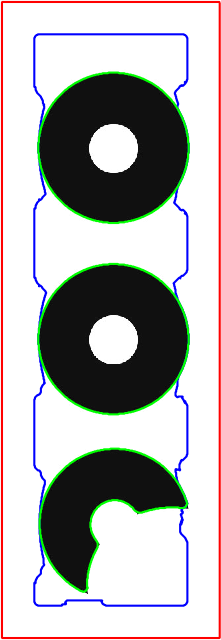
\includegraphics[scale=0.5]{figures/chapter2/segmentation/geodesic-seg.png}
}\hspace{2em}%
\subfloat[Chan-Vese]{
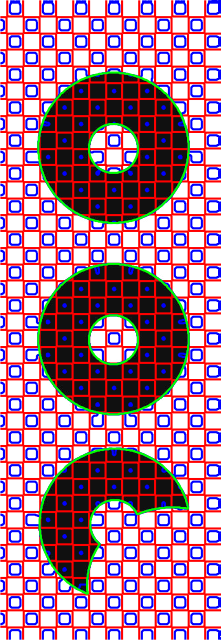
\includegraphics[scale=0.5]{figures/chapter2/segmentation/chan-vese-seg.png}
}%
\caption{Illustration of evolution curve models. The initial curve ($0$-level set) is colored in red and the final one is colored in green.}
\label{ch1:fig:comparison-curve-evolution}
\end{figure}


\subsection{Chan-Vese}
	The active contour and GAC are both edge-based methods, a natural strategy but with some limitations, e.g., the models may encounter some difficulties to segment objects with holes. The \emph{Chan-Vese} method proposes the inclusion of a region-based term and it generalizes the level-set rational of GAC. 
	
	Let $f_I:\Omega \subset \mathbb{R}^2 \rightarrow \mathbb{U}^2$ a grayscale image and $F \subset \Omega$ an open set such that the pair $(F,\Omega \setminus F)$ is the searched binary partition. Further, let us assume that there exists a function $\phi: \Omega \rightarrow \mathbb{R}$ with bounded first derivative. The image partitions are identified in the following fashion
	
\begin{align*}
	\phi(x) > 0,&\quad \forall x \in F \\
	\phi(x) = 0,&\quad \forall x \in \partial F\\
	\phi(x) < 0,&\quad \forall x \in \Omega \setminus \overline{F}
\end{align*}
	
	In possession of the partition descriptor $\phi$, the following energy is proposed	
	
\begin{align}
	F(\phi,x) &= \mu Length(\phi,x) + \nu Area(\phi,x) + \lambda_1 Foreground(\phi,x) + \lambda_2 Background(\phi,x) \nonumber \\	
	&= \mu \int_{\Omega}{\delta_0(\phi(x))\norm{ \nabla \phi(x)}dx} + \nu \int_{\Omega}{H(\phi(x))dx} \nonumber \\
	&+ \lambda_1 \int_{\Omega}{H(\phi(x))\norm{f - c_F}^2dx} + \lambda_2\int_{\Omega}{(1-H(\phi(x))\norm{f-c_B}^2dx},
	\label{ch1:eq:chan-vese-functional}
\end{align}

where $H(x)$ is the Heaviside function and $\delta_0$ the standard Dirac delta function, i.e.,

\[
\begin{array}{ll}
	H(x) = \left\{ \begin{array}{ll}
		1, & x \geq 0 \\
		0, & \text{otherwise},
	\end{array}\right. & \quad 
	
	\delta_0( x ) = \left\{ \begin{array}{ll}
								+ \infty,& x=0\\
								0,& \text{otherwise}.
							\end{array}\right. \text{ and } \int_{-\infty}^{+\infty}{\delta_0(x)dx}=1.
	
\end{array}
\]

The parameters $c_f,c_b$ are defined as the average color intensity in the interior of the foreground and background regions, respectively

\[
\begin{array}{ll}
	\displaystyle c_F = \frac{\int_{\Omega}{H(\phi(x))f(x)dx}}{\int_{\Omega}{H(\phi(x))dx}}, & 	
	\displaystyle c_B = \frac{\int_{\Omega}{(1-H(\phi(x)))f(x)dx}}{\int_{\Omega}{(1-H(\phi(x)))dx}}.
\end{array}
\]

Next, the Euler-Lagrange equation of~\cref{ch1:eq:chan-vese-functional} is calculated and used to define a gradient flow that aims to minimize~\cref{ch1:eq:chan-vese-functional}, in a similar fashion as done in~\cref{ch1:subsec:tikhonov-regularization}. In order to be numerically tractable, the Heaviside and Dirac delta function are regularized as 

\[
\begin{array}{ll}

	\begin{array}{ll}
		\displaystyle H_{\epsilon}(x) &= \displaystyle \frac{1}{2}\left( 1 + \frac{2}{\pi}\arctan(\frac{x}{\epsilon}) \right),
	\end{array} & 
	
	\begin{array}{ll}
		\displaystyle \delta_{\epsilon}(x) &= \displaystyle \frac{\epsilon}{\pi(\epsilon^2 + x^2)}.
	\end{array}	

\end{array}
\]

The initial level set function can be set as any function with bounded first derivative, but it is reported~\cite{getreuer12} that the checkerboard function $\phi=\sin(\pi/5 x_1)\sin(\pi/5x_2)$ presents fast convergence. 

Some examples of the Chan-Vese results for grayscale images are shown in~\ref{}. In~\cite{vese02}, the Chan-Vese authors extended their method to contemplate colored images and multisegmentation. 




%Relation with the minimal partition problem, whose solution existence has been proven, and piecewise constant MS  


\subsection{Geodesic active contours}

In a sequel work, the authors of GAC established a link between their geometric model in~\cite{caselles93} and the computation of geodesics in a regular surface~\cite{caselles97}. 

The length of a parametric curve $C(q)$ accordingly with an isotropic metric of potential $W(C)$ is calculated as 

\begin{align}
	L(C) &= \int{W(C)\norm{C_q} dq}.
	\label{ch1:eq:length-isotropic-metric}
\end{align}

~\cref{ch1:eq:length-isotropic-metric} is used to compute shortest paths between two points accordingly to the given metric. By properly setting the potential $W$, we can make object boundaries to match the curves of shortest length, for example, letting $W=g(\norm{\nabla f_I}^2)$ as in~\cref{ch1:geometric-active-contour} we obtain

\begin{align}
	L(C) &= \int{g\big(\norm{\nabla f_I(C(q))}\big)\norm{C_q} dq}.
	\label{ch1:eq:geodesic-energy}
\end{align}

In~\cite{caselles97} shows that active contour model without the smoothness term($\beta=0$) are equivalent to geodesics computations, the metric changing accordingly with the models parameters. The isotropic metric above is equivalent to the case in which the internal and external energies of the snakes are equal.

Given an initial curve $C_0(q)$, a local minimizer for~\cref{ch1:eq:geodesic-energy} can be computed by finding the steady solution of the following flow derived from its Euler-Lagrange equation

\begin{align}
	C(0,q) &= C_0(q)\\
	\frac{dC}{dt} &= (g\kappa - \nabla g \cdot \vec{n})\vec{n},
	\label{ch1:eq:curve-evolution}
\end{align}

where $\vec{n}$ is the normal vector to the curve $C$ at $(t,q)$. One can show that, given an initial function $u \in \mathcal{C}^2$ such that $u$ is negative (positive) in the interior (exterior) of its $0$-level set, the solution of~\cref{ch1:eq:curve-evolution} equals the steady solution of

\begin{align}
	u(0,x,y) &= u_0(x,y) \\
	\frac{du}{dt} &= g\norm{\nabla u}\kappa + \nabla g \cdot \nabla u
	\label{ch1:eq:surface-evolution}
\end{align}

Comparing~\cref{ch1:eq:surface-evolution} with~\cref{ch1:geometric-active-contour} we notice that the $\nabla g \cdot y$ term was included while the $v$ parameter was removed. The geometric active contour stops as soon as an ideal edge is found (a threshold should be set), which is particularly bad for real images segmentation, as it is likely the flow to stop at some outlier (noise) pixel. The new term allows the flow to evolve even in those cases. Nonetheless, one can include again the $v$ parameter, as it permits to increase the convergence in some cases.

The geodesic equivalence inspired several works that follows. Isotropic metrics were derived to segment roads~\cite{} and blood vessels~\cite{}. The role of anisotropic metrics is discussed in~\cite{} and an anisotropic metric is devised to segment MMM in~\cite{}.

%Taking the derivative of $\bar{u}$ at t$
%
%\begin{align*}
%	\bar{u}' &= 0\\
%	\frac{d\bar{u}}{dt} + \frac{d\bar{u}}{dx}\frac{dx}{dt} + \frac{d\bar{u}}{dy}\frac{dy}{dt} &= 0 \\
%	\frac{d\bar{u}}{dt} &= - \nabla u^{(t)} \cdot \nabla C^{(t)}
%\end{align*}
%
%For every level set of $u^{(t)}$ we have
%\begin{align*}
%	\frac{\nabla u^{(t)}}{\norm{\nabla u ^{(t)}}} &= -\vec{n}.
%\end{align*}
%Replacing in we obtain
%
%\begin{align*}
%	\frac{d\bar{u}}{dt} &= \norm{\nabla u^{(t)} } \vec{n} \cdot \nabla C^{(t)}
%\end{align*}




\section{Image inpainting}
\subsection{Level sets completion}



%There is an equivalence between Gibbs distributions and MRF.
%
%Maximum a posteriori is also called penalized maximum likelihood
%
%Consider the problem to find $x$ such that $Ax=b$. If the problem has none or several solutions, the problem is said do be ill-posed. The standard method to solve it is by least-squares plus a penalty term. $|Ax-b|^2 + \lambda P$. The term $P$ models a preference for solutions with some desirable property, e.g., $P=|x|^2$ will favor solutions with lower norm.
%
%Tikhonov regularization is a type of L2 regularization. It is known to improve the problem conditioning and to enable direct solutions (wikipedia article).